\documentclass[a4paper,10pt,fleqn]{article}

\usepackage{layout}



\begin{document}

\subsubsection*{Bezeichnung des LZI-Übertragungsgliedes}
\[ PT_2 \]

\subsubsection*{Übertragungsfunktion $G(s)$}
\[ \frac{4}{3 s^2 + 2 s + 1} \]

\subsubsection*{Stabilität des Übertragungsgliedes (Pole, Nulstellen, Plan)}
Nullstellen: keine, da $s$ im Zähler nicht vorkommt. \\\\
Polstellen: 
\[ 3 s^2 + 2 s + 1 = \left(s + \frac{1}{3} - \frac{\sqrt{2}}{3}j\right) \cdot \left(s + \frac{1}{3} + \frac{\sqrt{2}}{3}j\right) \]
\[ \rightarrow s_1 = -\frac{1}{3} + \frac{\sqrt{2}}{3}j \qquad s_2 = -\frac{1}{3} - \frac{\sqrt{2}}{3} \]

\subsubsection*{Zugehörige Differentialgleichung}

\subsubsection*{Berechnung der Einheitssprungantwort (Übertragungsfunktion) ($G(s)$, $H(s)$, $PBZ$, $L^-1$, $h(t)$, Skizze)}

\subsubsection*{Berechnung und Skizze des Bode-Diagramms ($G(j\omega)$, $|G(j\omega)|_{dB}$, $arc(G(j\omega))$)}
\begin{figure}[h!]
\center
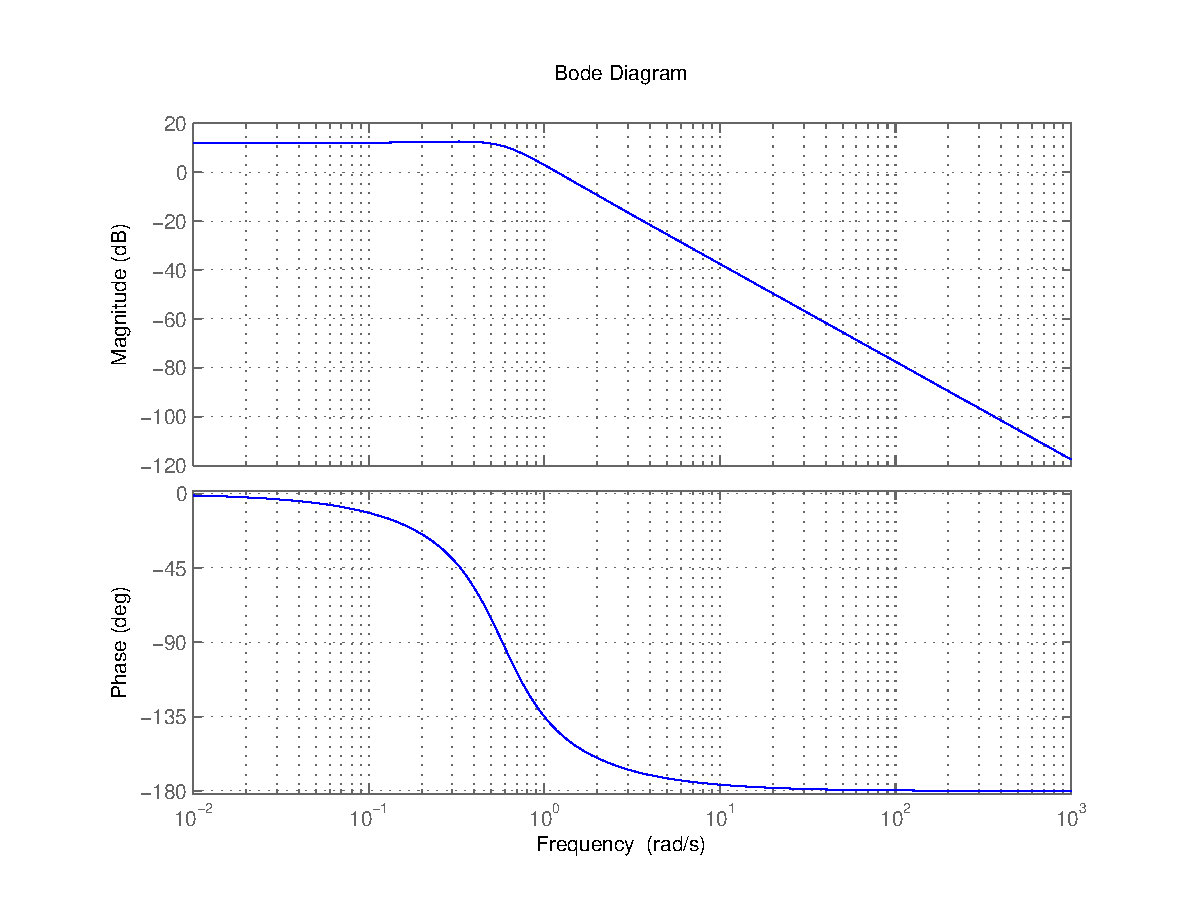
\includegraphics[width=\textwidth]{bode.eps}
\end{figure}

\subsection*{Skizze der Nyquist Ortskurve ($G(j\omega)$)}
\begin{figure}[h!]
\center
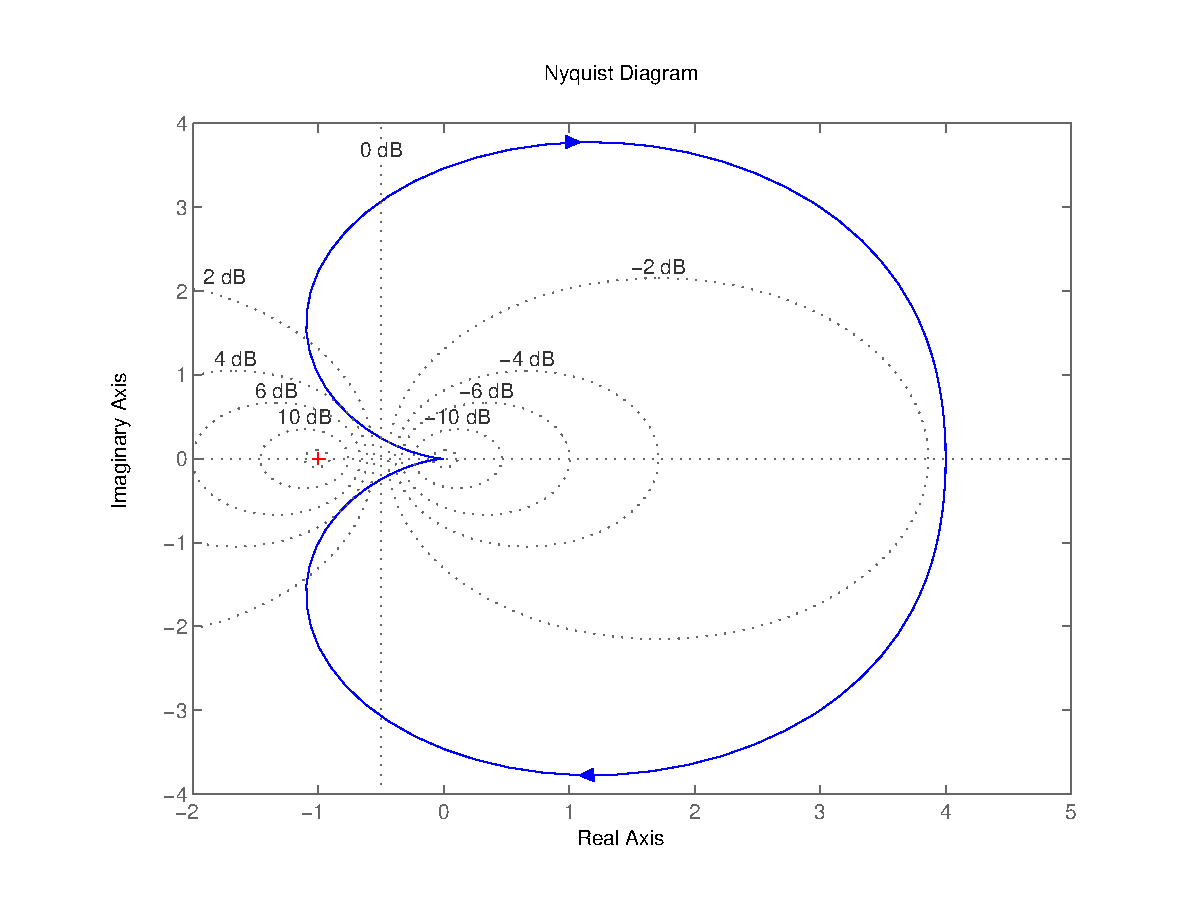
\includegraphics[width=\textwidth]{nyquist.eps}
\end{figure}

\end{document}
